% answers.tex —— 2007 年·普通高等学校招生考试·陕西卷·文科 · 参考答案与详细解析片段
% 由 tools/generate_projects.py 依来源总账自 2007/2007_数学真题_陕西文_试题.md + 2007/2007_数学真题_陕西文_解析正文.md + 2007/2007_数学真题_陕西文_答案要点.md 生成，勿手改（改源 MD 后重跑）


\begin{gktip}
固定候选 PDF 仅含题面，无答案、解析和评分标准，原卷亦未标注分值；以下为非官方编者独立推导，官方答案字段为空。来源发布者、出版者、版次与官方身份均未核。
\end{gktip}

\begin{answer}
\gksolhead{1}{}

\textbf{题目}：

已知全集 $U=\{1,2,3,4,5,6\}$，集合 $A=\{2,3,6\}$，则集合 $\complement_UA$ 等于（　）

（A）$\{1,4\}$

（B）$\{4,5\}$

（C）$\{1,4,5\}$

（D）$\{2,3,6\}$

\Needspace{4\baselineskip}
\textbf{解析}

\Needspace{5\baselineskip}
$U=\{1,2,3,4,5,6\}$，$A=\{2,3,6\}$，故

\nopagebreak[4]
\[\complement_UA=\{1,4,5\}.\]

\gkanswer{答案：C。}

\end{answer}
\begin{answer}
\gksolhead{2}{}

\textbf{题目}：

函数 $f(x)=\lg\sqrt{1-x^2}$ 的定义域为（　）

（A）$[0,1]$

（B）$(-1,1)$

（C）$[-1,1]$

（D）$(-\infty,-1)\cup(1,+\infty)$

\Needspace{4\baselineskip}
\textbf{解析}

\Needspace{5\baselineskip}
根号内为正：

\nopagebreak[4]
\[1-x^2>0\ \Rightarrow\ -1<x<1.\]

\gkanswer{答案：B。}

\end{answer}
\begin{answer}
\gksolhead{3}{}

\textbf{题目}：

抛物线 $x^2=y$ 的准线方程是（　）

（A）$4x+1=0$

（B）$4y+1=0$

（C）$2x+1=0$

（D）$2y+1=0$

\Needspace{4\baselineskip}
\textbf{解析}

\Needspace{5\baselineskip}
$x^2=y$ 即 $x^2=2py$ 中 $p=\dfrac12$，准线

\nopagebreak[4]
\[y=-\frac p2=-\frac14\ \Rightarrow\ 4y+1=0.\]

\gkanswer{答案：B。}

\end{answer}
\begin{answer}
\gksolhead{4}{}

\textbf{题目}：

已知 $\sin\alpha=\dfrac{\sqrt5}{5}$，则 $\sin^4\alpha-\cos^4\alpha$ 的值为（　）

（A）$-\frac35$

（B）$-\frac15$

（C）$\frac15$

（D）$\frac35$

\Needspace{4\baselineskip}
\textbf{解析}

\nopagebreak[4]
\[\sin^4\alpha-\cos^4\alpha=(\sin^2\alpha-\cos^2\alpha)(\sin^2\alpha+\cos^2\alpha)\]

\nopagebreak[4]
\[=2\sin^2\alpha-1=2\cdot\frac15-1=-\frac35.\]

\gkanswer{答案：A。}

\end{answer}
\begin{answer}
\gksolhead{5}{}

\textbf{题目}：

等差数列 $\{a_n\}$ 的前 $n$ 项和为 $S_n$，若 $S_2=2$，$S_4=10$，则 $S_6$ 等于（　）

（A）$12$

（B）$18$

（C）$24$

（D）$42$

\Needspace{4\baselineskip}
\textbf{解析}

\Needspace{5\baselineskip}
等差数列中 $S_2$，$S_4-S_2$，$S_6-S_4$ 成等差数列，即

\nopagebreak[4]
\[2,\ 8,\ S_6-10\]

\Needspace{5\baselineskip}
成等差数列。由等差中项

\nopagebreak[4]
\[2\times8=2+(S_6-10),\]

\Needspace{5\baselineskip}
得

\nopagebreak[4]
\[S_6-10=14\ \Rightarrow\ S_6=24.\]

\gkanswer{答案：C。}

\end{answer}
\begin{answer}
\gksolhead{6}{}

\textbf{题目}：

某商场有四类食品，其中粮食类、植物油类、动物性食品类以及果蔬类分别有 $40$ 种、$10$ 种、$30$ 种、$20$ 种，现从中抽取一个容量为 $20$ 的样本进行食品安全检测。若采用分层抽样的方法抽取样本，则抽取的植物油类与果蔬类食品种数之和是（　）

（A）$4$

（B）$5$

（C）$6$

（D）$7$

\Needspace{4\baselineskip}
\textbf{解析}

\Needspace{5\baselineskip}
抽样比为 $\dfrac{20}{100}=\dfrac15$。植物油类抽取

\nopagebreak[4]
\[10\times\frac15=2,\]

\Needspace{5\baselineskip}
果蔬类抽取

\nopagebreak[4]
\[20\times\frac15=4,\]

合计 $6$。

\gkanswer{答案：C。}

\end{answer}
\begin{answer}
\gksolhead{7}{}

\textbf{题目}：

$\mathrm{Rt}\triangle ABC$ 的三个顶点在半径为 $13$ 的球面上，直角边的长分别为 $6$ 和 $8$，则球心到平面 $ABC$ 的距离是（　）

（A）$5$

（B）$6$

（C）$10$

（D）$12$

\Needspace{4\baselineskip}
\textbf{解析}

\Needspace{5\baselineskip}
直角三角形斜边为

\nopagebreak[4]
\[\sqrt{6^2+8^2}=10,\]

\Needspace{5\baselineskip}
其外接圆半径为 $5$。球心到平面 $ABC$ 的距离

\nopagebreak[4]
\[d=\sqrt{13^2-5^2}=\sqrt{144}=12.\]

\gkanswer{答案：D。}

\end{answer}
\begin{answer}
\gksolhead{8}{}

\textbf{题目}：

设函数 $f(x)=2^x+1$（$x\in\mathbf R$）的反函数为 $f^{-1}(x)$，则函数 $y=f^{-1}(x)$ 的图象是（　）
\nopagebreak[4]
\begin{center}% 2007 年陕西卷文科第 8 题：反函数 y=log2(x-1) 的图象选项。
%   （D）为正确图象，其余为定义域/平移不同的干扰项。
% 来源 PDF：gaokaomath-src/普通高考/2007/2007陕西文.pdf
% SHA-256：95abaa3050f33e9b9587ad186af8f173fbf40c31ebe3f2be710bbae607ed0ecb
% 原页：2007陕西文.pdf 第 1 页（A3 三栏）第 2 栏，书页码 403。
% 重绘依据：按原页四个小图的曲线、渐近线与截距重绘。
\begin{tikzpicture}[scale=0.85, semithick,
  every node/.style={inner sep=1pt, font=\small}]
  % A：只画 x>=2 一支
  \begin{scope}[shift={(0,0)}]
    \draw[->,>=stealth] (-0.4,0) -- (2.6,0) node[right] {$x$};
    \draw[->,>=stealth] (0,-1.4) -- (0,1.8) node[above] {$y$};
    \draw[dashed] (1,-1.4) -- (1,1.8);
    \draw[domain=2:2.5,samples=60] plot (\x,{ln(\x-1)/ln(2)});
    \node[below] at (0.7,-1.8) {（A）};
  \end{scope}
  % B：平移错误
  \begin{scope}[shift={(4.3,0)}]
    \draw[->,>=stealth] (-0.4,0) -- (2.6,0) node[right] {$x$};
    \draw[->,>=stealth] (0,-1.4) -- (0,1.8) node[above] {$y$};
    \draw[dashed] (1,-1.4) -- (1,1.8);
    \draw[domain=1.05:2.5,samples=60] plot (\x,{ln(\x)/ln(2)});
    \node[below] at (0.7,-1.8) {（B）};
  \end{scope}
  % C：y=log2 x
  \begin{scope}[shift={(0,-4.0)}]
    \draw[->,>=stealth] (-0.4,0) -- (2.6,0) node[right] {$x$};
    \draw[->,>=stealth] (0,-1.4) -- (0,1.8) node[above] {$y$};
    \draw[dashed] (0,-1.4) -- (0,1.8);
    \draw[domain=0.2:2.5,samples=60] plot (\x,{ln(\x)/ln(2)});
    \node[below] at (0.7,-1.8) {（C）};
  \end{scope}
  % D：正确
  \begin{scope}[shift={(4.3,-4.0)}]
    \draw[->,>=stealth] (-0.4,0) -- (2.6,0) node[right] {$x$};
    \draw[->,>=stealth] (0,-1.4) -- (0,1.8) node[above] {$y$};
    \draw[dashed] (1,-1.4) -- (1,1.8);
    \draw[domain=1.05:2.5,samples=60] plot (\x,{ln(\x-1)/ln(2)});
    \node[below] at (0.7,-1.8) {（D）};
  \end{scope}
\end{tikzpicture}
\end{center}
\nopagebreak[4]
\Needspace{4\baselineskip}
\textbf{解析}

\Needspace{5\baselineskip}
$y=2^x+1$ 的反函数为

\nopagebreak[4]
\[y=\log_2(x-1),\]

定义域 $x>1$，过 $(2,0)$，竖直渐近线 $x=1$，在 $(1,2)$ 上为负。选项 D 符合。

\gkanswer{答案：D。}

\end{answer}
\begin{answer}
\gksolhead{9}{}

\textbf{题目}：

已知双曲线 $C$：$\dfrac{x^2}{a^2}-\dfrac{y^2}{b^2}=1$（$a>0$，$b>0$），以 $C$ 的右焦点为圆心且与 $C$ 的渐近线相切的圆的半径是（　）

（A）$a$

（B）$b$

（C）$\sqrt{ab}$

（D）$\sqrt{a^2+b^2}$

\Needspace{4\baselineskip}
\textbf{解析}

\Needspace{5\baselineskip}
渐近线 $bx-ay=0$，右焦点 $(c,0)$ 到渐近线的距离

\nopagebreak[4]
\[r=\frac{|bc|}{\sqrt{a^2+b^2}}=b.\]

\gkanswer{答案：B。}

\end{answer}
\begin{answer}
\gksolhead{10}{}

\textbf{题目}：

已知 $P$ 为平面 $\alpha$ 外一点，直线 $l\subset\alpha$，点 $Q\in l$，记点 $P$ 到平面 $\alpha$ 的距离为 $a$，点 $P$ 到直线 $l$ 的距离为 $b$，点 $P$，$Q$ 之间的距离为 $c$，则（　）

（A）$a\leqslant b\leqslant c$

（B）$c\leqslant a\leqslant b$

（C）$a\leqslant c\leqslant b$

（D）$b\leqslant c\leqslant a$

\Needspace{4\baselineskip}
\textbf{解析}

\Needspace{5\baselineskip}
$P$ 到平面的距离是到平面内任一点距离的最小值，故 $a\leqslant c$；$P$ 到直线 $l$ 的距离是到 $l$ 上点距离的最小值，故 $b\leqslant c$；又 $l\subset\alpha$，点到平面的距离不超过到平面内直线的距离，故 $a\leqslant b$。因此

\nopagebreak[4]
\[a\leqslant b\leqslant c.\]

\gkanswer{答案：A。}

\end{answer}
\begin{answer}
\gksolhead{11}{}

\textbf{题目}：

给出如下三个命题：

① 设 $a$，$b\in\mathbf R$，且 $ab\neq0$，若 $\dfrac ab>1$，则 $\dfrac ba<1$；

② 四个非零实数 $a$，$b$，$c$，$d$ 依次成等比数列的充要条件是 $ad=bc$；

③ 若 $f(x)=\log_2x$，则 $f(|x|)$ 是偶函数。

其中正确命题的序号是（　）

（A）①②

（B）②③

（C）①③

（D）①②③

\Needspace{4\baselineskip}
\textbf{解析}

① $\dfrac ab>1>0$，故 $a$，$b$ 同号且 $|a|>|b|$，于是 $0<\dfrac ba<1$，真。

② $ad=bc$ 不足以保证依次成等比，如 $1,2,2,4$，假。

③ $f(|x|)=\log_2|x|$，定义域关于原点对称且为偶函数，真。

\gkanswer{答案：C。}

\end{answer}
\begin{answer}
\gksolhead{12}{}

\textbf{题目}：

某生物生长过程中，在三个连续时段内的增长量都相等，在各时段内平均增长速度分别为 $v_1$，$v_2$，$v_3$，该生物在所讨论的整个时段内的平均增长速度为（　）

（A）$\frac{v_1+v_2+v_3}{3}$

（B）$\frac{\frac1{v_1}+\frac1{v_2}+\frac1{v_3}}{3}$

（C）$\sqrt[3]{v_1v_2v_3}$

（D）$\frac3{\frac1{v_1}+\frac1{v_2}+\frac1{v_3}}$

\Needspace{4\baselineskip}
\textbf{解析}

\Needspace{5\baselineskip}
设每段增长量为 $\Delta$，三段用时分别为 $\dfrac{\Delta}{v_1}$，$\dfrac{\Delta}{v_2}$，$\dfrac{\Delta}{v_3}$。总平均速度

\nopagebreak[4]
\[\bar v=\frac{3\Delta}{\frac{\Delta}{v_1}+\frac{\Delta}{v_2}+\frac{\Delta}{v_3}}
=\frac3{\frac1{v_1}+\frac1{v_2}+\frac1{v_3}}.\]

\gkanswer{答案：D。}

\end{answer}
\begin{answer}
\gksolhead{13}{}

\textbf{题目}：

$(1+2x)^5$ 的展开式中 $x^2$ 项的系数是\gkblank{}。（用数字作答）

\Needspace{4\baselineskip}
\textbf{解析}

\nopagebreak[4]
\[\mathrm C_5^2\cdot2^2=10\times4=40.\]

\gkanswer{答案：$40$。}

\end{answer}
\begin{answer}
\gksolhead{14}{}

\textbf{题目}：

已知实数 $x$，$y$ 满足条件 $\begin{cases}x-2y+4\geqslant0,\\ 3x-y-3\leqslant0,\\ x\geqslant0,\ y\geqslant0,\end{cases}$ 则 $z=x+2y$ 的最大值为\gkblank{}。

\Needspace{4\baselineskip}
\textbf{解析}

\Needspace{5\baselineskip}
可行域的三个顶点为 $(0,0)$，$(0,2)$，$(1,0)$，以及两直线交点 $(2,3)$。计算

\nopagebreak[4]
\[z=x+2y:\quad (0,0)\to0,\ (0,2)\to4,\ (1,0)\to1,\ (2,3)\to8.\]

最大值为 $8$。

\gkanswer{答案：$8$。}

\end{answer}
\begin{answer}
\gksolhead{15}{}

\textbf{题目}：

安排 $3$ 名支教教师去 $4$ 所学校任教，每校至多 $2$ 人，则不同的分配方案共有\gkblank{}种。（用数字作答）

\Needspace{4\baselineskip}
\textbf{解析}

\Needspace{5\baselineskip}
不加限制共有 $4^3=64$ 种。某校分到 $3$ 人的情况有 $4$ 种（选择该校），其余分配均满足每校至多 $2$ 人。故

\nopagebreak[4]
\[64-4=60.\]

\gkanswer{答案：$60$。}

\end{answer}
\begin{answer}
\gksolhead{16}{}

\textbf{题目}：

如图，平面内有三个向量 $\overrightarrow{OA}$，$\overrightarrow{OB}$，$\overrightarrow{OC}$，其中 $\overrightarrow{OA}$ 与 $\overrightarrow{OB}$ 的夹角为 $120^\circ$，$\overrightarrow{OA}$ 与 $\overrightarrow{OC}$ 的夹角为 $30^\circ$，且 $|\overrightarrow{OA}|=|\overrightarrow{OB}|=1$，$|\overrightarrow{OC}|=2\sqrt3$。若 $\overrightarrow{OC}=\lambda\overrightarrow{OA}+\mu\overrightarrow{OB}$（$\lambda$，$\mu\in\mathbf R$），则 $\lambda+\mu$ 的值为\gkblank{}。
\nopagebreak[4]
\begin{center}% 2007 年陕西卷文科第 16 题：向量 OA、OB、OC 的夹角关系。
%   OA 与 OB 成 120°，OA 与 OC 成 30°，|OA|=|OB|=1，|OC|=2√3。
% 来源 PDF：gaokaomath-src/普通高考/2007/2007陕西文.pdf
% SHA-256：95abaa3050f33e9b9587ad186af8f173fbf40c31ebe3f2be710bbae607ed0ecb
% 原页：2007陕西文.pdf 第 1 页（A3 三栏）第 3 栏，书页码 403。
% 重绘依据：按原页三个向量的方向与长度比例重绘。
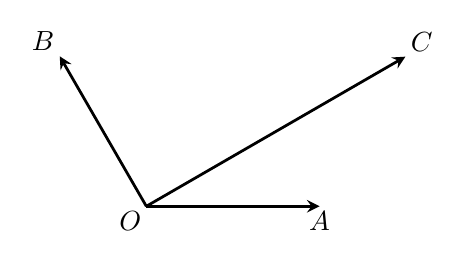
\begin{tikzpicture}[scale=1.0, semithick,
  every node/.style={inner sep=1.5pt}]
  \coordinate (O) at (0,0);
  \coordinate (A) at (2.2,0);
  \coordinate (B) at (-1.1,1.905);
  \coordinate (C) at (3.29,1.9);

  \draw[->,>=stealth,line width=1pt] (O) -- (A) node[below] {$A$};
  \draw[->,>=stealth,line width=1pt] (O) -- (B) node[above left] {$B$};
  \draw[->,>=stealth,line width=1pt] (O) -- (C) node[above right] {$C$};
  \node[below left] at (O) {$O$};
\end{tikzpicture}
\end{center}
\nopagebreak[4]
\Needspace{4\baselineskip}
\textbf{解析}

\Needspace{5\baselineskip}
设 $\overrightarrow{OA}$ 为 $x$ 轴方向，则 $\overrightarrow{OB}$ 与它成 $120^\circ$，$\overrightarrow{OC}$ 与它成 $30^\circ$（方向在两者之间）。由

\nopagebreak[4]
\[\overrightarrow{OC}\cdot\overrightarrow{OA}=2\sqrt3\cos30^\circ=3,\]

\nopagebreak[4]
\[\overrightarrow{OC}\cdot\overrightarrow{OB}=2\sqrt3\cos90^\circ=0.\]

\Needspace{5\baselineskip}
而 $\overrightarrow{OC}=\lambda\overrightarrow{OA}+\mu\overrightarrow{OB}$，故

\nopagebreak[4]
\[3=\lambda+\mu\cos120^\circ=\lambda-\frac\mu2,\]

\nopagebreak[4]
\[0=\lambda\cos120^\circ+\mu=-\frac\lambda2+\mu.\]

\Needspace{5\baselineskip}
由第二式 $\mu=\dfrac\lambda2$，代入第一式：

\nopagebreak[4]
\[\lambda-\frac\lambda4=3\ \Rightarrow\ \frac{3\lambda}4=3\ \Rightarrow\ \lambda=4,\ \mu=2.\]

故 $\lambda+\mu=6$。

\gkanswer{答案：$6$。}

\end{answer}
\begin{answer}
\gksolhead{17}{}

\textbf{题目}：

设函数 $f(x)=\boldsymbol a\cdot\boldsymbol b$，其中向量 $\boldsymbol a=(m,\cos x)$，$\boldsymbol b=(1+\sin x,1)$，$x\in\mathbf R$，且 $f\left(\dfrac{\pi}{2}\right)=2$。

（1）求实数 $m$ 的值；

（2）求函数 $f(x)$ 的最小值。

\Needspace{4\baselineskip}
\textbf{解析}

\Needspace{5\baselineskip}
（1）

\nopagebreak[4]
\[f(x)=m(1+\sin x)+\cos x.\]

\Needspace{5\baselineskip}
由 $f\left(\dfrac{\pi}{2}\right)=2$：

\nopagebreak[4]
\[m(1+1)+0=2\ \Rightarrow\ m=1.\]

\Needspace{5\baselineskip}
（2）

\nopagebreak[4]
\[f(x)=1+\sin x+\cos x=1+\sqrt2\sin\left(x+\frac{\pi}{4}\right),\]

\Needspace{5\baselineskip}
故最小值为

\nopagebreak[4]
\[1-\sqrt2.\]

\gkanswer{答案：（1）$m=1$；（2）最小值 $1-\sqrt2$。}

\end{answer}
\begin{answer}
\gksolhead{18}{}

\textbf{题目}：

某项选拔共有四轮考核，每轮设有一个问题，能正确回答问题者进入下一轮考核，否则即被淘汰。已知某选手能正确回答第一、二、三、四轮的问题的概率分别为 $\dfrac45$，$\dfrac35$，$\dfrac25$，$\dfrac15$，且各轮问题能否正确回答互不影响。

（1）求该选手进入第四轮才被淘汰的概率；

（2）求该选手至多进入第三轮考核的概率。

\Needspace{4\baselineskip}
\textbf{解析}

\Needspace{5\baselineskip}
（1）进入第四轮才被淘汰＝前三轮都答对、第四轮答错：

\nopagebreak[4]
\[P=\frac45\cdot\frac35\cdot\frac25\cdot\left(1-\frac15\right)
=\frac{24}{125}\cdot\frac45=\frac{96}{625}.\]

\Needspace{5\baselineskip}
（2）“至多进入第三轮”即没有进入第四轮，其对立事件是前三轮全对：

\nopagebreak[4]
\[P=1-\frac45\cdot\frac35\cdot\frac25=1-\frac{24}{125}=\frac{101}{125}.\]

\gkanswer{答案：（1）$\dfrac{96}{625}$；（2）$\dfrac{101}{125}$。}

\end{answer}
\begin{answer}
\gksolhead{19}{}

\textbf{题目}：

如图，在底面为直角梯形的四棱锥 $P-ABCD$ 中，$AD\parallel BC$，$\angle ABC=90^\circ$，$PA\perp$ 平面 $ABCD$，$PA=3$，$AD=2$，$AB=2\sqrt3$，$BC=6$。

（1）求证：$BD\perp$ 平面 $PAC$；

（2）求二面角 $P-BD-A$ 的大小。
\nopagebreak[4]
\begin{center}% 2007 年陕西卷文科第 19 题：底面为直角梯形的四棱锥 P-ABCD，PA⊥底面。
%   AD∥BC，∠ABC=90°，PA=3，AD=2，AB=2√3，BC=6；E 为 AC 与 BD 的交点。
% 来源 PDF：gaokaomath-src/普通高考/2007/2007陕西文.pdf
% SHA-256：95abaa3050f33e9b9587ad186af8f173fbf40c31ebe3f2be710bbae607ed0ecb
% 原页：2007陕西文.pdf 第 2 页（A3 三栏）第 1 栏，书页码 404。
% 重绘依据：按原页底面梯形、P 的位置与 E 点重绘。
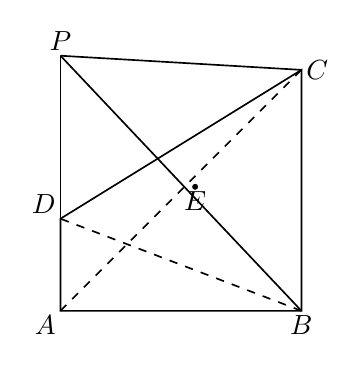
\begin{tikzpicture}[scale=0.9, semithick,
  every node/.style={inner sep=1.5pt}]
  \coordinate (A) at (0,0);
  \coordinate (B) at (3.4,0);
  \coordinate (C) at (3.4,3.4);
  \coordinate (D) at (0,1.3);
  \coordinate (P) at (0,3.6);
  \coordinate (E) at (1.9,1.75);

  \draw (A) -- (B) -- (C) -- (D) -- cycle;
  \draw (P) -- (A);
  \draw (P) -- (B);
  \draw (P) -- (C);
  \draw (P) -- (D);
  \draw[dashed] (A) -- (C);
  \draw[dashed] (B) -- (D);
  \fill (E) circle (1.2pt);

  \node[below left] at (A) {$A$};
  \node[below] at (B) {$B$};
  \node[right] at (C) {$C$};
  \node[above left] at (D) {$D$};
  \node[above] at (P) {$P$};
  \node[below] at (E) {$E$};
\end{tikzpicture}
\end{center}
\nopagebreak[4]
\Needspace{4\baselineskip}
\textbf{解析}

\Needspace{5\baselineskip}
以 $A$ 为原点，$AB$，$AD$，$AP$ 为 $x$，$y$，$z$ 轴：

\nopagebreak[4]
\[A(0,0,0),\ B(2\sqrt3,0,0),\ C(2\sqrt3,6,0),\ D(0,2,0),\ P(0,0,3).\]

\Needspace{5\baselineskip}
（1）

\nopagebreak[4]
\[\overrightarrow{BD}=(-2\sqrt3,2,0),\qquad \overrightarrow{AC}=(2\sqrt3,6,0).\]

\nopagebreak[4]
\[\overrightarrow{BD}\cdot\overrightarrow{AC}=-12+12=0,\]

\Needspace{5\baselineskip}
故 $BD\perp AC$。又 $PA\perp$ 底面，故 $PA\perp BD$。$AC$ 与 $PA$ 相交于 $A$，所以

\nopagebreak[4]
\[BD\perp\text{\text{平面} }PAC.\]

\Needspace{5\baselineskip}
（2）平面 $ABD$（即底面）的法向量为 $(0,0,1)$。平面 $PBD$ 内

\nopagebreak[4]
\[\overrightarrow{DB}=(2\sqrt3,-2,0),\qquad \overrightarrow{DP}=(0,-2,3).\]

\Needspace{5\baselineskip}
法向量

\nopagebreak[4]
\[\boldsymbol n=\overrightarrow{DB}\times\overrightarrow{DP}=(-6,-6\sqrt3,-4\sqrt3)\sim(3,3\sqrt3,2\sqrt3).\]

\Needspace{5\baselineskip}
设二面角为 $\theta$，则

\nopagebreak[4]
\[\cos\theta=\frac{2\sqrt3}{\sqrt{9+27+12}}=\frac{2\sqrt3}{4\sqrt3}=\frac12,\]

\Needspace{5\baselineskip}
故

\nopagebreak[4]
\[\theta=60^\circ.\]

\gkanswer{答案：（1）证明见解析；（2）$60^\circ$。}

\end{answer}
\begin{answer}
\gksolhead{20}{}

\textbf{题目}：

已知实数 $\{a_n\}$ 是等比数列，其中 $a_7=1$，且 $a_4$，$a_5+1$，$a_6$ 成等差数列。

（1）求数列 $\{a_n\}$ 的通项公式；

（2）数列 $\{a_n\}$ 的前 $n$ 项和记为 $S_n$，证明：$S_n<128$（$n=1,2,3,\cdots$）。

\Needspace{4\baselineskip}
\textbf{解析}

\Needspace{5\baselineskip}
（1）设 $a_n=Aq^{n-1}$。由 $a_7=1$ 得 $Aq^6=1$。又 $a_4$，$a_5+1$，$a_6$ 成等差数列：

\nopagebreak[4]
\[2(Aq^4+1)=Aq^3+Aq^5.\]

\Needspace{5\baselineskip}
两边除以 $Aq^3$，并利用 $\dfrac1{Aq^3}=q^3$：

\nopagebreak[4]
\[2(q+q^3)=1+q^2,\]

\nopagebreak[4]
\[2q^3-q^2+2q-1=0,\]

\nopagebreak[4]
\[(2q-1)(q^2+1)=0.\]

\Needspace{5\baselineskip}
故 $q=\dfrac12$，$A=64$，即

\nopagebreak[4]
\[a_n=64\left(\frac12\right)^{n-1}=2^{7-n}.\]

\Needspace{5\baselineskip}
（2）前 $n$ 项和

\nopagebreak[4]
\[S_n=\frac{64\left(1-2^{-n}\right)}{1-\frac12}=128(1-2^{-n})<128.\]

\gkanswer{答案：（1）$a_n=2^{7-n}$；（2）证明见解析。}

\end{answer}
\begin{answer}
\gksolhead{21}{}

\textbf{题目}：

已知 $f(x)=ax^3+bx^2+cx$ 在区间 $[0,1]$ 上是增函数，在区间 $(-\infty,0)$，$(1,+\infty)$ 上是减函数。又 $f'\left(\dfrac12\right)=\dfrac32$。

（1）求 $f(x)$ 的解析式；

（2）若在区间 $[0,m]$（$m>0$）上恒有 $f(x)\leqslant x$ 成立，求 $m$ 的取值范围。

\Needspace{4\baselineskip}
\textbf{解析}

\Needspace{5\baselineskip}
（1）$f'(x)=3ax^2+2bx+c$。由单调性，$f'$ 在 $x=0$，$x=1$ 处变号，且开口向下，故

\nopagebreak[4]
\[f'(x)=k x(1-x)\quad(k>0).\]

\Needspace{5\baselineskip}
于是 $c=0$，$2b=k$，$3a=-k$。又

\nopagebreak[4]
\[f'\left(\frac12\right)=k\cdot\frac12\cdot\frac12=\frac k4=\frac32,\]

\Needspace{5\baselineskip}
故 $k=6$，从而

\nopagebreak[4]
\[a=-2,\qquad b=3,\qquad c=0,\]

\nopagebreak[4]
\[f(x)=-2x^3+3x^2.\]

\Needspace{5\baselineskip}
（2）

\nopagebreak[4]
\[f(x)-x=-2x^3+3x^2-x=x(1-x)(2x-1).\]

\Needspace{5\baselineskip}
在 $[0,m]$ 上要求 $f(x)\leqslant x$，即

\nopagebreak[4]
\[x(1-x)(2x-1)\leqslant0.\]

当 $0<x<\dfrac12$ 时，$1-x>0$，$2x-1<0$，乘积为负，符合；当 $\dfrac12<x<1$ 时乘积为正，不符合；当 $x\geqslant1$ 时，$1-x\leqslant0$，$2x-1>0$，乘积为负，符合。

\Needspace{5\baselineskip}
故区间 $[0,m]$ 不能越过 $\dfrac12$，即

\nopagebreak[4]
\[0<m\leqslant\frac12.\]

\gkanswer{答案：（1）$f(x)=-2x^3+3x^2$；（2）$0<m\leqslant\dfrac12$。}

\end{answer}